In this Chapter we report the results of the training and validation of the neural networks described in the experimental approach. Then, we discuss the results in terms of the research questions defined. Lastly, we assess the validity and limitations of our experimental procedure and results

\section{Experiment Result}
\begin{table}	
	\centering
	\begin{tabular}{ |c|c|c|c|c| } 
		\hline
		& MNIST & Fashion MNIST & CIFAR-10 & SVHN \\ 
		\hline
		LeNet-5	& 0.9834 & 0.8816 & 0.6561 & 0.809\\
		\hline 
		VGG-like & 0.9946 & 0.91 & 0.4075 & 0.067\\ 
		\hline
		Resnet20v1 & 0.9246 & 0.592 & 0.7567 & 0.866\\ 
		\hline
		Resnet20v2 & 0.9222 & 0.8425 & 0.679 & 0.893\\
		\hline
		SqueezeNet & 0.9858 & 0.8813 & 0.555 & 0.775\\
		\hline
	\end{tabular}
	\label{tab:accuracy}
	\caption{Accuracy table}
\end{table}

\begin{table}
	\centering
	\begin{tabular}{ |c|c|c|c|c| } 
		\hline
		& MNIST & Fashion MNIST & CIFAR-10 & SVHN \\ 
		\hline
		LeNet-5	& 220s & 220s & 330s & 220s\\
		\hline 
		VGG-like & 4986s	& 4469s & 6816s & 6526s\\ 
		\hline
		Resnet20v1 & 7970s & 7909s	& 7204s & 9310s\\ 
		\hline
		Resnet20v2 & 13900s & 	13910s & 	12060s & 	15693s\\
		\hline
		SqueezeNet & 13800s & 	13907s & 	13630s & 	17550s\\
		\hline
	\end{tabular}
	%\caption{Execution time for each experiment.}
	\label{tab:times}
	\caption{Execution time table}
\end{table}
Table \ref{tab:accuracy} shows the result of the experiments in terms of accuracy. The execution times and number of parametes for each experiment is shown on \ref{tab:times} \ref{fig:params}.



\begin{figure}[h]
	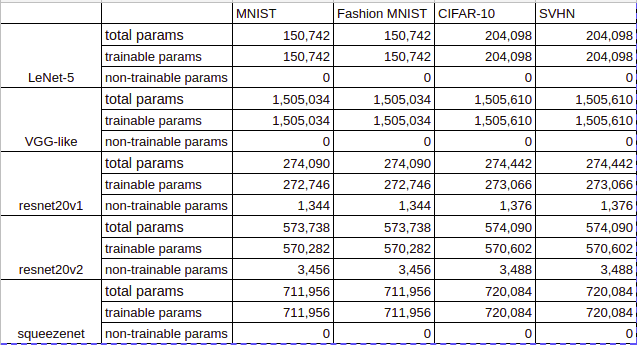
\includegraphics[scale=0.5]{figures/params}
	\centering
	\caption{Number of parameters for each experiment.}
	\label{fig:params}
\end{figure}

\section{Discussion}
In this Chapter, we reported the results of the experiments to answer the following research questions that was previously stated:

"How does the performance comparison of deep learning architecture model looks like for a given image classification dataset?"

\begin{enumerate}
	\item Which architecture that works bests for a given datasets?
	
	From table \ref{tab:accuracy}, we can see that VGG-like architecture performs the best on MNIST and Fashion MNIST dataset. ResNet20V1 and ResNet20V2 performs the best on CIFAR-10 and SVHN dataset respectively. In terms of memory usage and time consumption, it is proven that LeNet produces the simplest for all datasets.
	
	
	\item What kind of datasets characteristics that makes a deep learning architecture works well?
	
	From table \ref{tab:accuracy}, we can see that 
	\item Is there any architecture that generally works well for image classification?	
\end{enumerate}


 